\documentclass[a4paper]{article}
\usepackage{amsmath}
\usepackage{graphicx}
\usepackage{geometry}
\usepackage{enumerate}
\usepackage{amssymb}
\usepackage{anyfontsize}
\usepackage{indentfirst}
\usepackage[font=small,labelfont=bf]{caption}
\usepackage{subcaption}
\usepackage{latexsym}
\usepackage{threeparttable}
\usepackage{multirow}
\usepackage[colorlinks,urlcolor=blue]{hyperref}
\usepackage{minted}
\usemintedstyle{autumn}
\setminted{linenos,breaklines,tabsize=4,xleftmargin=1.5em}
\begin{document}
	\begin{titlepage}
	\vspace{200pt}


		\begin{center}
		\rule[0pt]{12cm}{0.05em}
		
		 \Large{UM-SJTU \quad JOINT \quad INSTITURE}
		 \vspace{8pt}
		
		 
		 Intro to Computer Organization
		 
		 (VE370)		 
		 
		 \rule[0pt]{12cm}{0.05em}
		 
		 \vspace{50pt}
		 
		  {\fontsize{15}{30}\selectfont \textbf{Project 1}}
		  \vspace{8pt}

		  {\fontsize{15}{30}\selectfont \textit{prof. Zheng}}
		  
		 
		 \vspace{250pt}

		 
		

		 
		XINMIAO YU 
		
		518021910792 
		\vspace{5pt}
		
		\vspace{80pt}
		 \end{center}
		 
		DATE: 28 Sept. 2020
	\end{titlepage}
	
	\pagestyle{plain}
	
	\section{Introduction}
In this project, an array of 32-bits signed integer has a predefined \textbf{size 32}. These 32 numbers are assigned randomly. The C program is shown below. 

\begin{minted}
[
frame=lines,
framesep=2mm,
linenos
]{C}
int main() {
    int size = 32; //determine the size of the array here 
    int hotDay, coldDay, comfortDay;
    int tempArray[32] = {36, 9, -8, 40, 25, 20, 18, 19, 15, 16, 17, 16, 15, 14, 
	13, 12, 11, 10, 9, 8, 7, 6, 5, 4, 3, 2, 1, 0, -3, 30, -19, 33};
    hotDay = countArray (tempArray, size, 1); 
    coldDay = countArray (tempArray, size, -1); 
    comfortDay = countArray (tempArray, size, 0);
}
int countArray(int A[], int numElements, int cntType) {
    int i, cnt = 0;
    for (i = numElements - 1; i >= 0; i--) {
        switch (cntType) {
            case 1: cnt += hot(A[i]); break;
            case -1: cnt += cold(A[i]); break;
            default: cnt += comfort(A[i]);
        }
    }
    return cnt;
}
int hot(int x) {
    if(x>=30) return 1;
    else return 0;
}
int cold(int x) {
    if (x<=5) return 1;
    else return 0;
}
int comfort(int x) {
    if (x>5 && x<30) return 1;
    else return 0;
}

\end{minted}
A MIPS program with same functions as the C program is developed. In addition, no pseudo-instruction used. 


	\section{Procedures}
The program is developed following the logic of C program. 
\begin{enumerate}
\item[•] As use \mintinline{C}{la} to load in the address of array is not allowed, the address used to store the numbers is predefined, as $0x10001000$. Then \mintinline{C}{main} function, where \mintinline{C}{int tempArray[32]=...} is needed, the base address ($0x10001000$) is load in \$a0 through the command \mintinline{C}{lui} and \mintinline{C}{ori}.
\item[•] In \mintinline{C}{main} function, other variables needed is defined as 



\begin{minted}{C}
$a1 = size			// as numElements = 32 
$s0 = hotDay 		// as 0
$s1 = coldDay 		// as 0
$s2 = comfortDay 	// as 0
 \end{minted}
function \mintinline{C}{countArray} is called three times. Before each call, make 
\$a2 as 1/-1/0 and the \textbf{stack pointer} is adjusted for 6 items. The function arguments (\$a0, \$a1), return address (\$ra) and saved register (\$s0, \$s1, \$s2) are all saved into the stack before call \mintinline{C}{countArray} and restored after the function call. According to the return value in \$v0, the number of hotDay/coldDay/comfortDay are all determined.
\item[•] In function \mintinline{C}{countArray}, define 
\begin{minted}{C}
$s0 = 0				// as numElements - 1 = 31 
$s1 = cnt 			// as 0
 \end{minted}
 Same as before, before function call adjust stack pointer for saving \$a0, \$a1, \$a2, \$ra, \$s0, \$s1. Set \$a0 = A[i], where the address of A[i] is obtained through \$a0 + \$s0 *4. 
 Restore all the value after each function call and change \$s1 according to the value in \$v0.
 \item[•] For leaf function \mintinline{C}{hot/cold/comfort}, return the right value, stored in \$v0. 
\end{enumerate}	
	
		
	\section{Simulation Result}
	The simulation result is obtained through \textit{QtSpim}. All the register show decimal value for simpler explanation. 
	\begin{enumerate}
	\item \textbf{Before first call \mintinline{C}{countArray}}
	
\begin{figure}[!ht]\centering
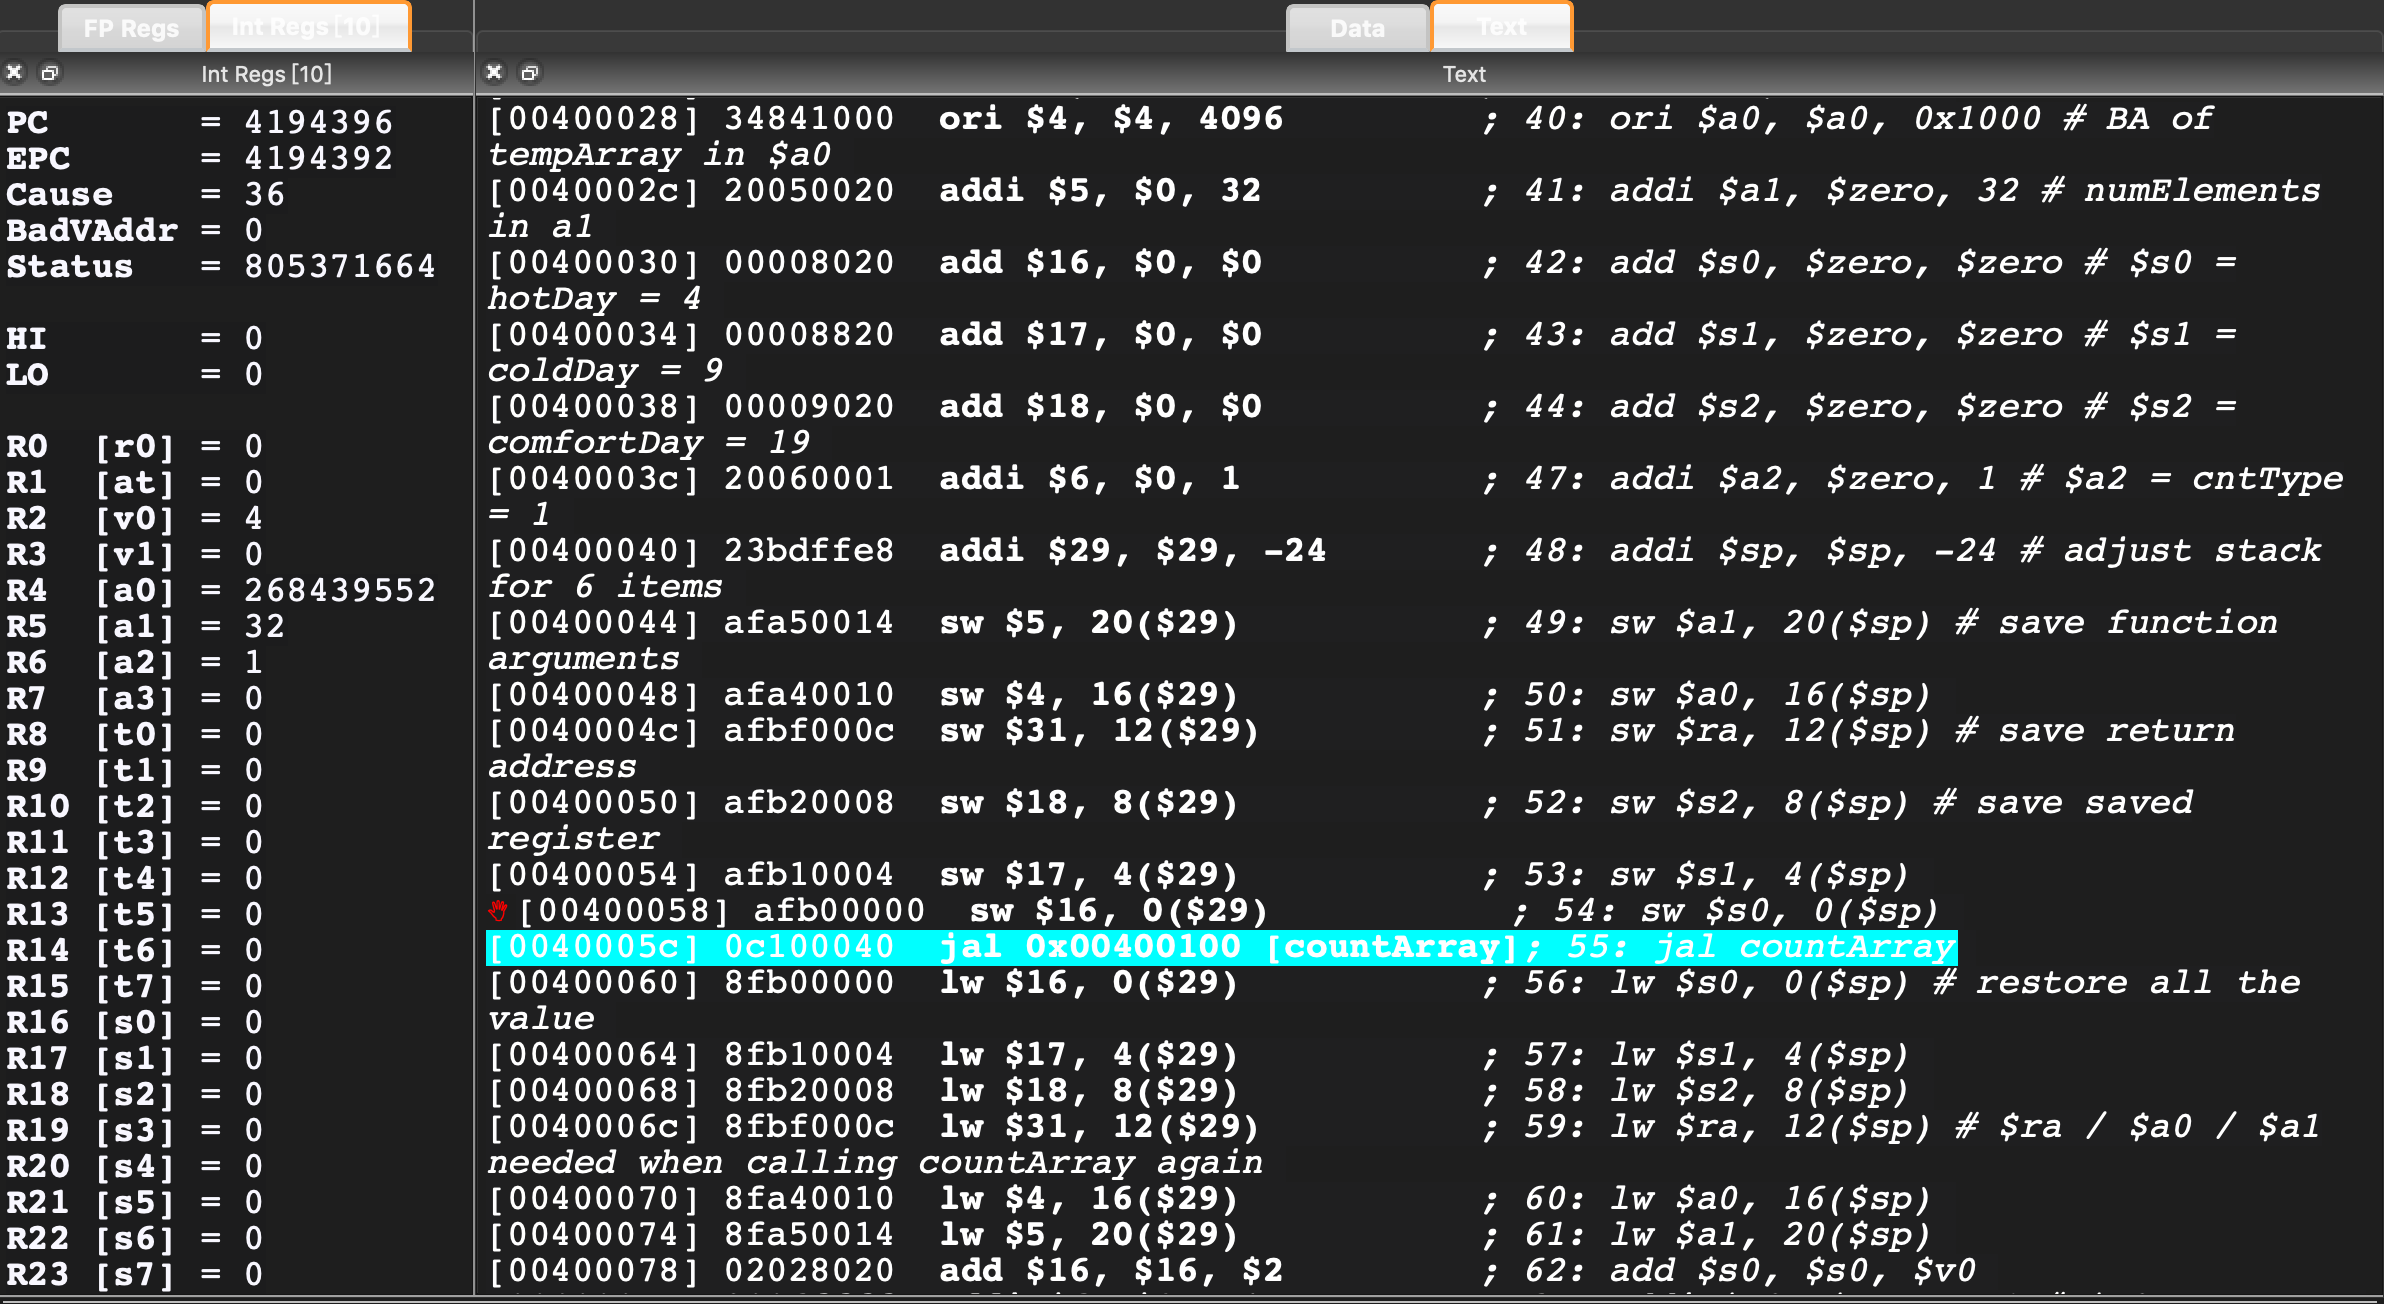
\includegraphics[scale=0.34]{/Users/yuxinmiao/Documents/JI/JI2020Fall/VE370/Projects/P1/screenshot/beforecount.png}
\label{before}
\end{figure}
we could see that \$a0 = (268439552)$_{10}$ = 0x10001000, \$a1 = 32, \$a2 = 1, as expected. 
\newpage
\item \textbf{Before first call \mintinline{C}{hot/cold/comfort}}


 \begin{figure}[!h]\centering
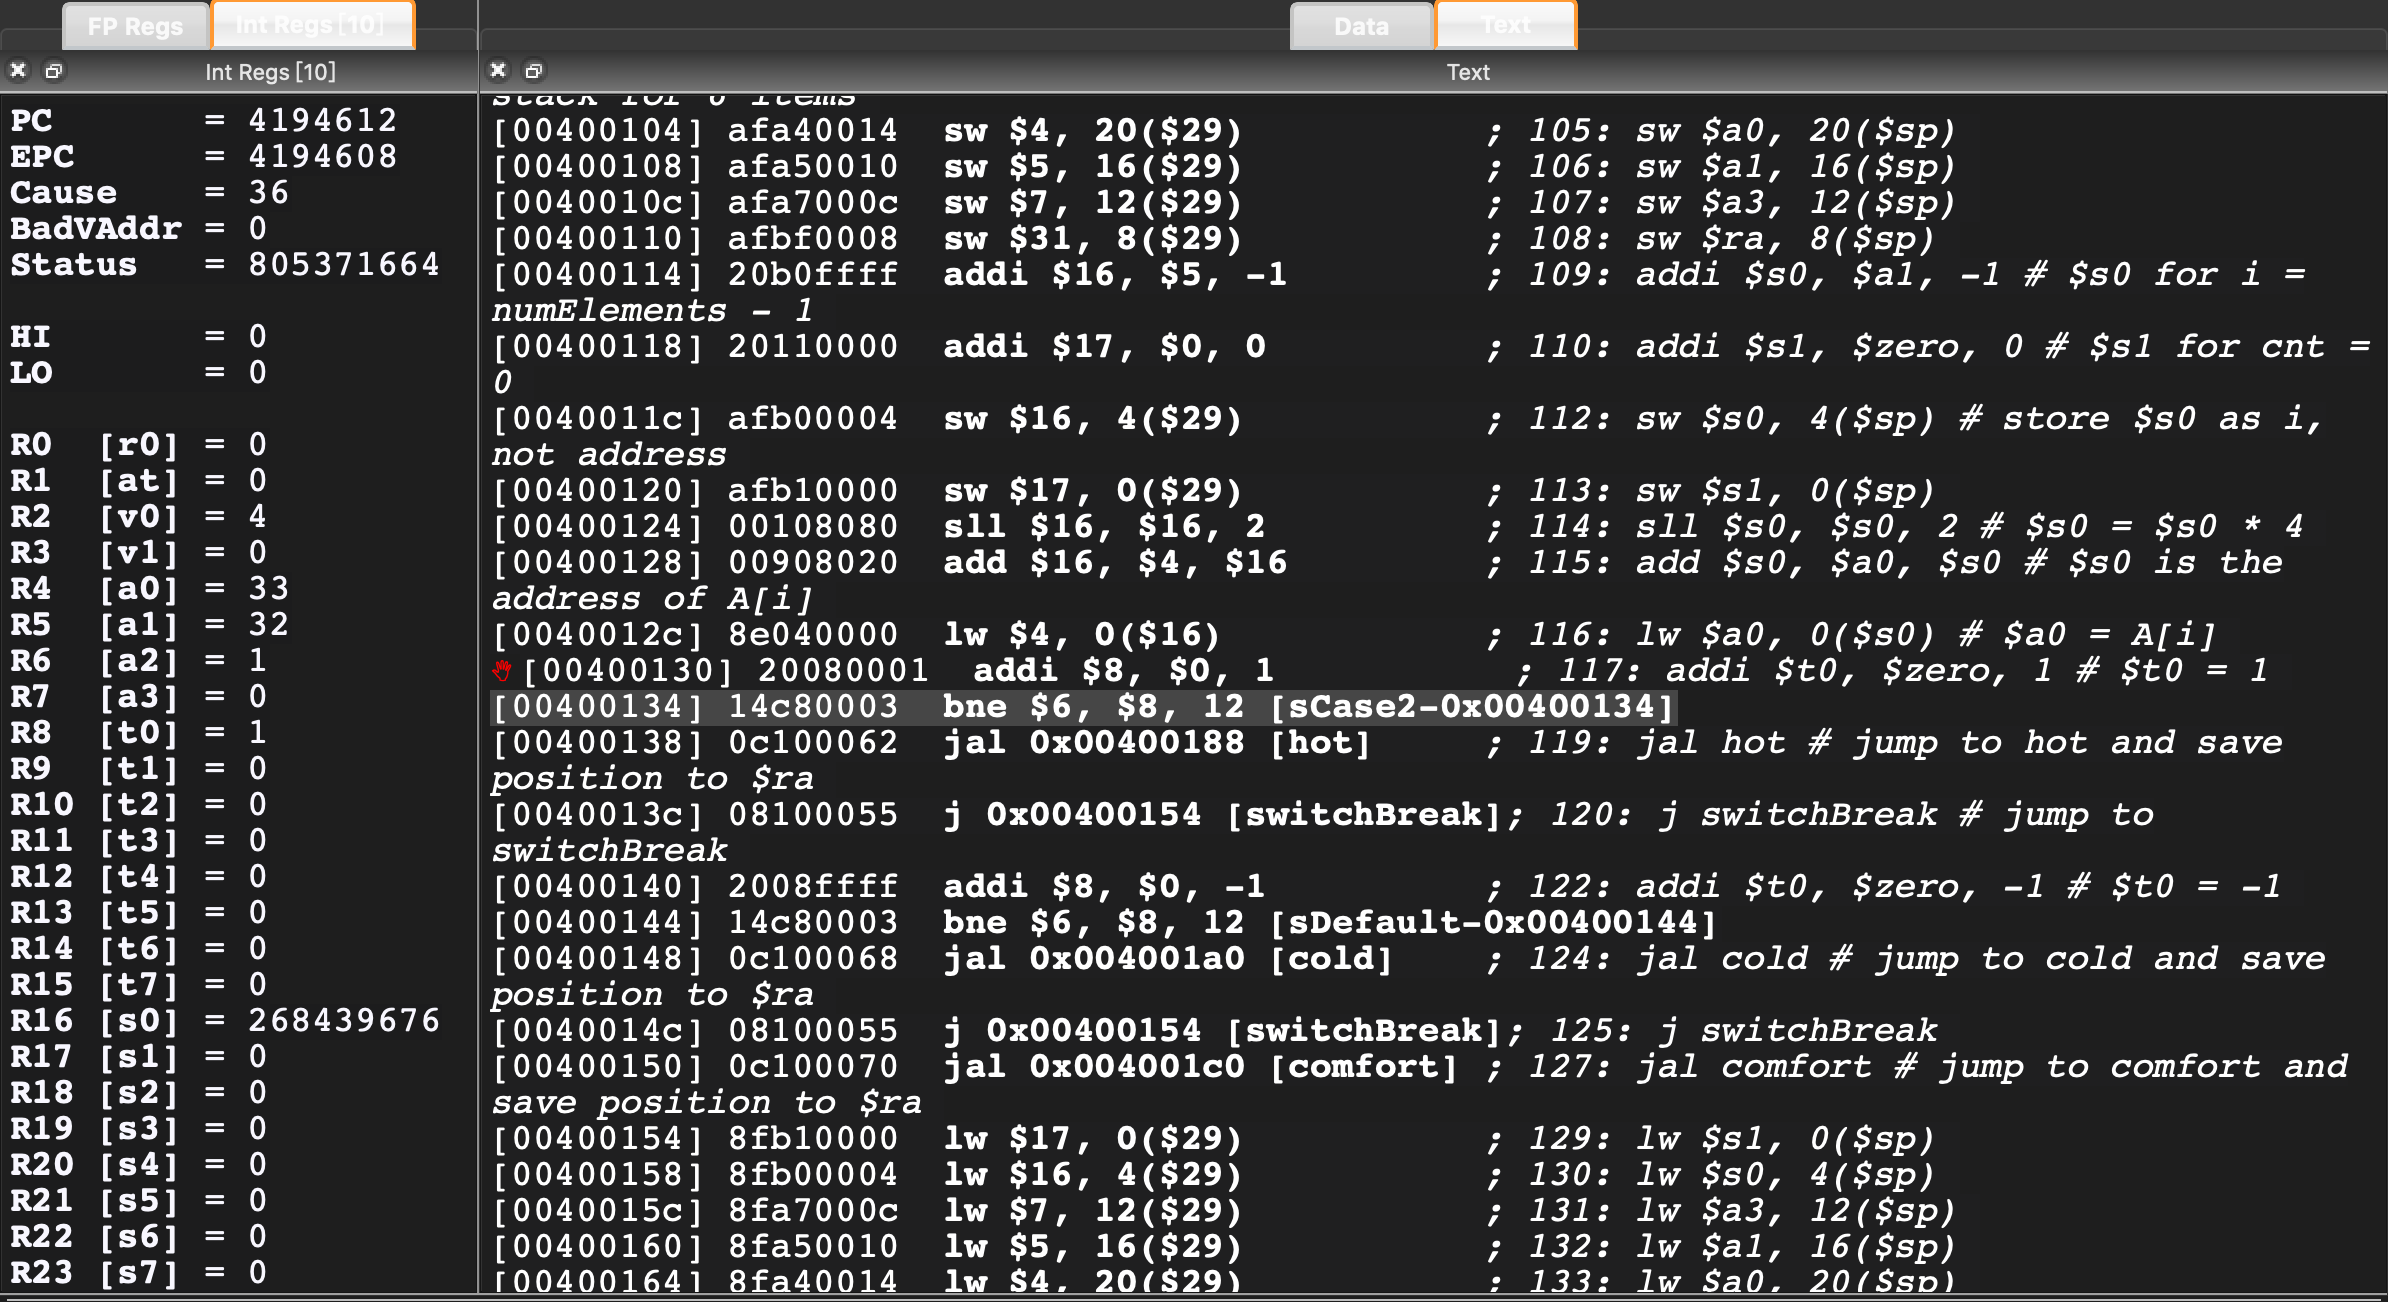
\includegraphics[scale=0.36]{/Users/yuxinmiao/Documents/JI/JI2020Fall/VE370/Projects/P1/screenshot/beforehot.png}
\label{before}
\end{figure}
the value of A[i], which is A[31] = 33, is load in \$a0, as function argument to pass to the leaf function. Now \$s0 has the address of A[31] = (268439676)$_{10}$ = 0x1000107c = 0x10001000 + (32 * 4)$_{10}$. Then the loop will continue until all the value in the array are passed. 

\item \textbf{After first call \mintinline{C}{countArray}}


 \begin{figure}[!h]\centering
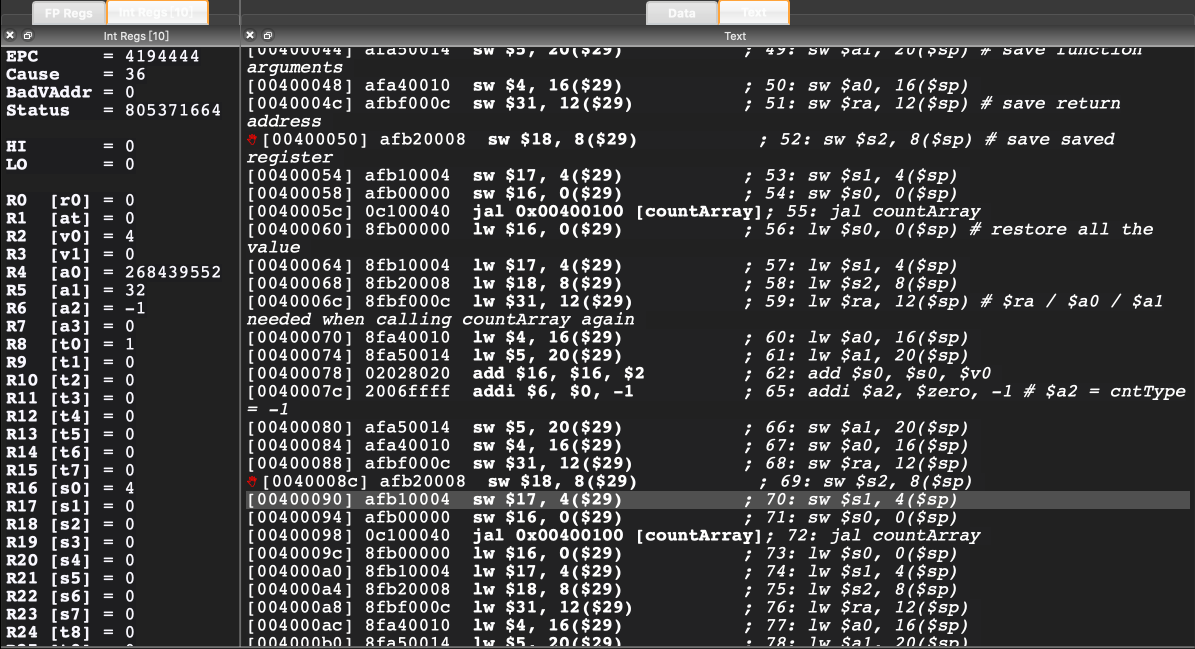
\includegraphics[scale=0.7]{/Users/yuxinmiao/Documents/JI/JI2020Fall/VE370/Projects/P1/screenshot/after.png}
\label{before}
\end{figure}
The value of hotDay is stored in \$s0, which is 4. \$a2 is set as -1 for count coldDay. The value of \$a0 and \$a1 should not change as restored from stack. Then the procedure is similar, only differ in the leaf function called. 

\item \textbf{Finish}

 \begin{figure}[!h]\centering
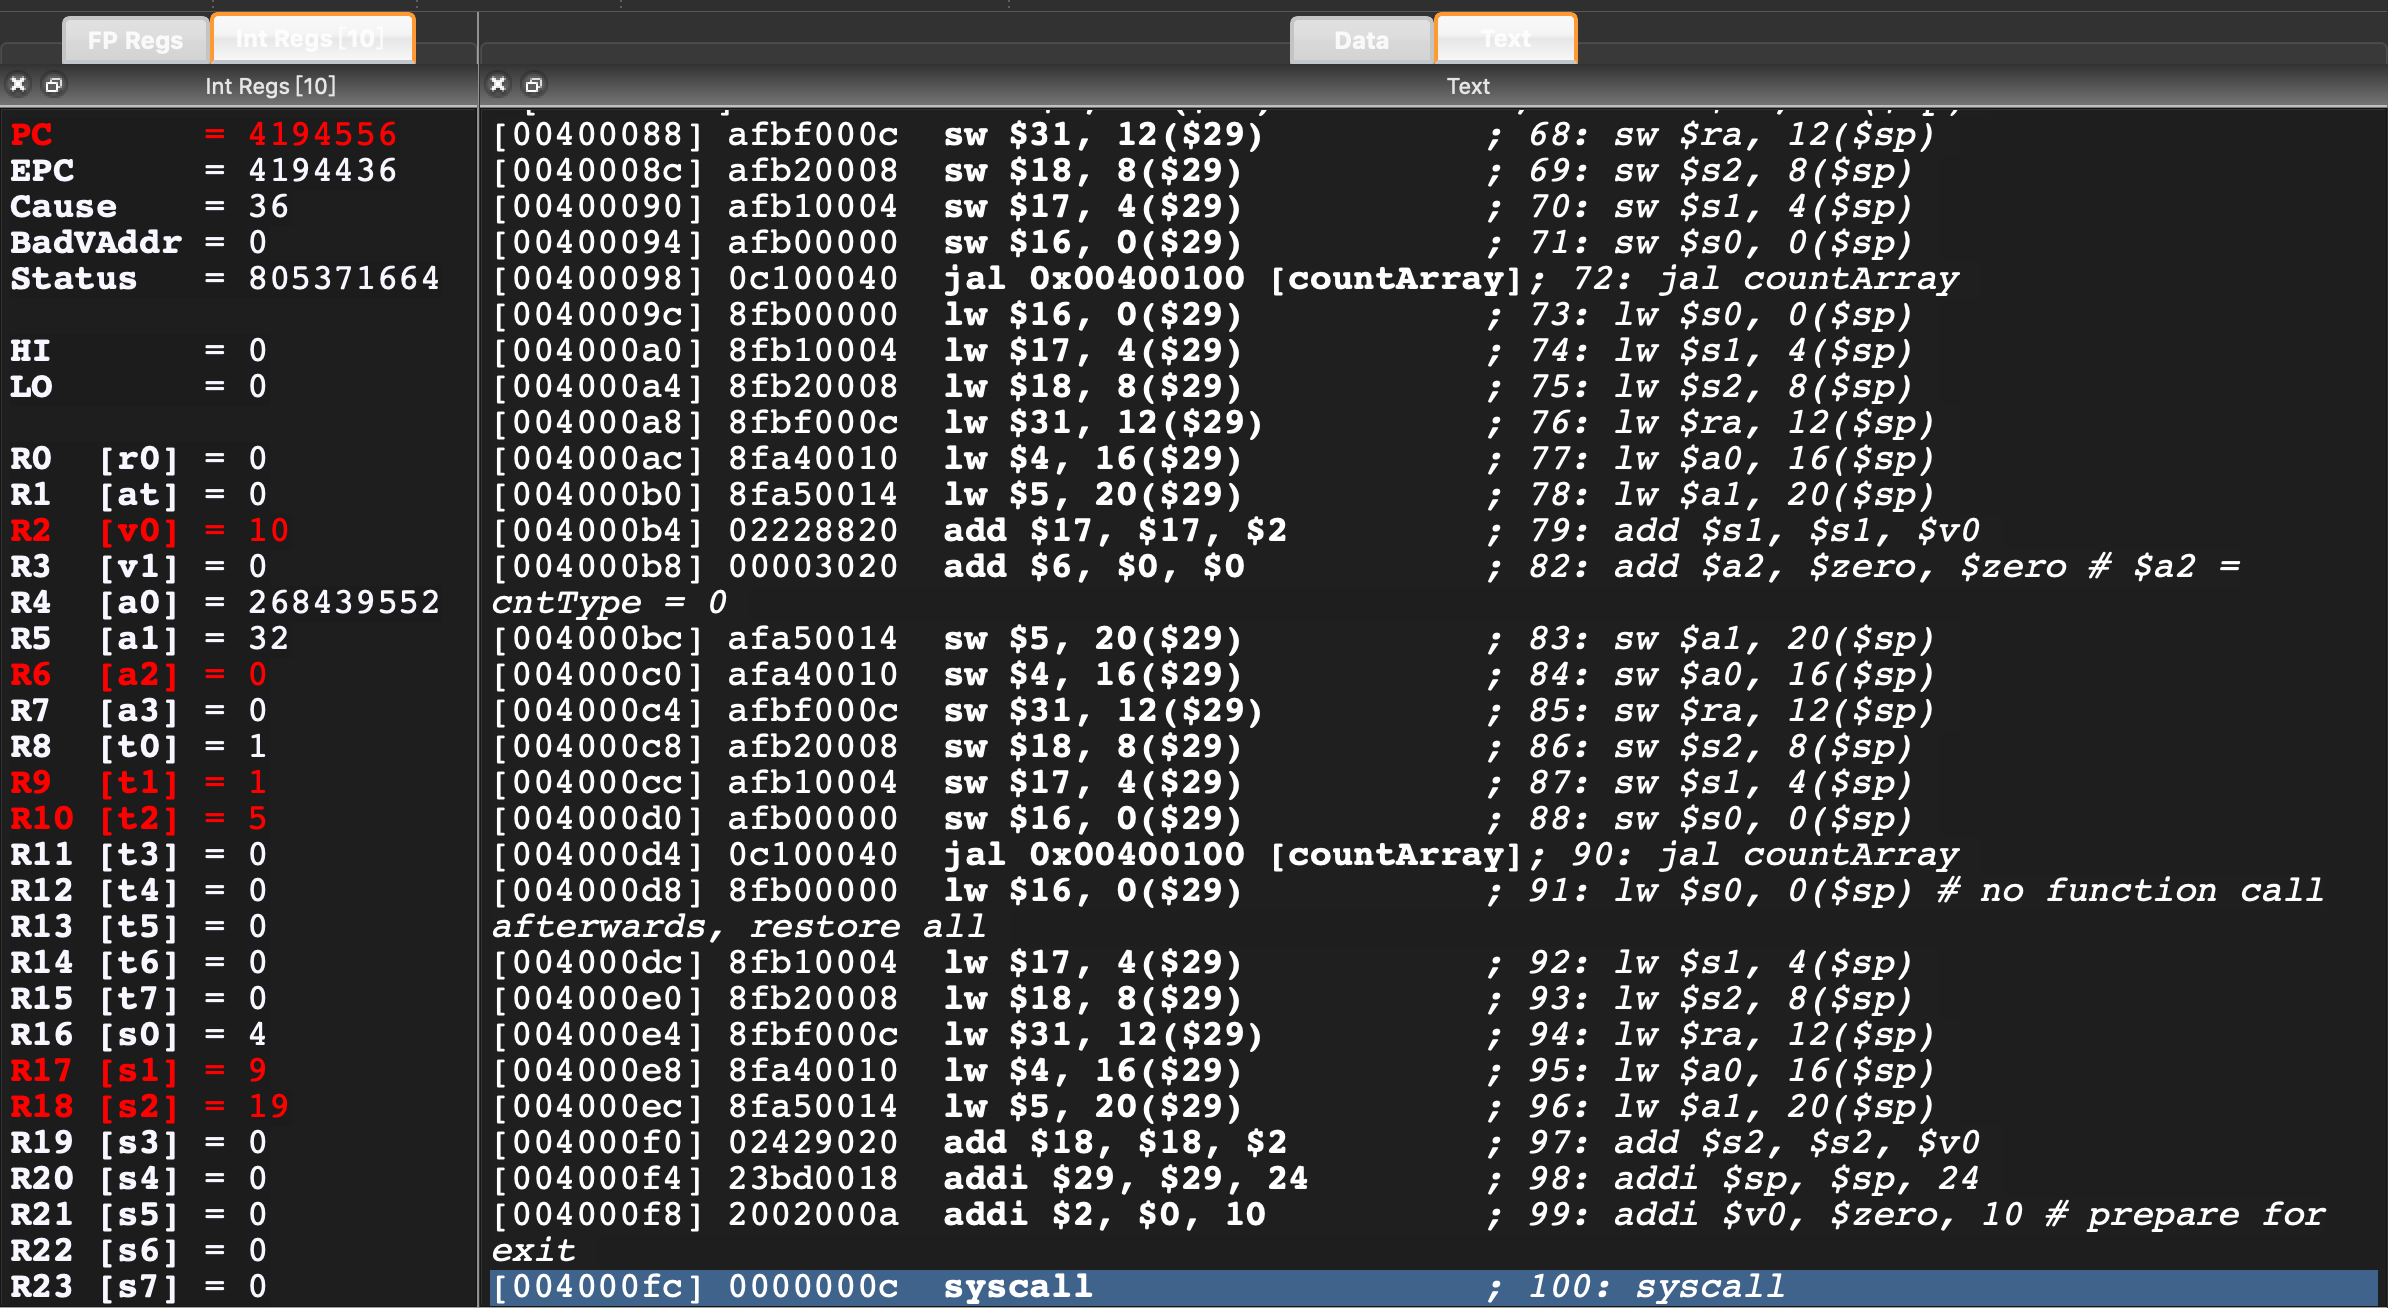
\includegraphics[scale=0.375]{/Users/yuxinmiao/Documents/JI/JI2020Fall/VE370/Projects/P1/screenshot/finish.png}
\label{before}
\end{figure}
	When the program finishes, \$s0 = 4 (the number of hotDays), \$s1 = 9 (the number of coldDays), \$s2 = 19 (the number of comfortDays), as expected. 
	
	\end{enumerate}
	
	\section{Conclusion}
	In conclusion, the program written through MIPS successfully finished the expected tasks and output the correct answer. Potential error might caused by
	\begin{enumerate}
	\item[•] use pseudo-instruction, caused syntax error.
	\item[•] forget to adjust the stack pointer to save/restore values before/after each function call.
	\item[•] the existed delay. Add some meaningless command will help. 

	\end{enumerate}

	\newpage	
	\appendix
	\section{Program}
\inputminted{asm}{p1.s}

	
\end{document}

